\sectionthree{Turing Machines}
\begin{python0}
from solutions import *; clear()
\end{python0}

Informally, a Turing machine (TM) is like a DFA or a PDA except for
the following:
\begin{itemize}
\item For the DFA (and PDA), the machines read the input string one
 character at a time from the leftmost character to the rightmost. A
 TM can also read the input one character at a time. However
 the input string should be thought of as being written on an
 infinitely long tape; you should think of the tape as being padded
 infinitely to the right with blanks. The TM can actually write to it
 as well. Therefore you should think of the TM as having a read/write
 head that moves along an infinitely long string.
 Furthermore, the read/write head can move either
 left or right or it can also stay. The only restriction is that it
 must stay on the infinitely tape.
\item For the DFA, acceptance is
 determined by what the state the machine is in once the string is
 completely read. For the TM, since the input string is written on an
 infinite tape, there is really no end-of-string. Therefore for a TM, a string is
 accepted if the machine enters an accepting state, regardless of the
 position of the read/write head.
\end{itemize}

Even without a formal definition of a TM, you probably know by now
that the most important thing about running the TM is that you need
to know what happens when the machine is in a particular state and
it is about to read a particular character. What if the machine
capable of doing? Well, obviously it has to go to another (possibly
the same) state. It can overwrite the character it is reading; this
is sort of like the PDA. Furthermore it can move it's read/write
head either to the left or right or it stays. So the transition
function should look like:

\[\delta(q, a) = (p, b, D)\]

where $q$ and $p$ are states, $a$ and $b$ are the allowable
characters on the infinite tape and $D$ refers to the direction
moved by the read/write head. $D$ can take values $L$ (for left),
$S$ (for stay) and $R$ (for right).

Here's the formal definition. Most of this won't be a surprise to
you by now. There's one thing I should mention. We will distinguish
between the alphabet of the string used to generate a language (the
$\Sigma$) and the alphabet that the TM can write on the tape.

\begin{defn}
A {\bf Turing machine} TM $M$ is made up of
\begin{itemize}
 \item $Q$: a finite set of states.
 \item $\Sigma$: a finite set of input alphabet.
 \item $\Gamma$: a finite set of alphabet the TM using for read and write.
 $\Sigma$ is a subset of $\Gamma$.
 Furthermore the blank character is also in $\Gamma$.
 \item $q_0$: the initial state. This is in $Q$.
 \item $F$: the set of accepting states. $F$ is a subset of $Q$.
 \item $R$: the set of reject states. $R$ is a subset of $Q$.
 \item $B$: the blank symbol; this is in $\Gamma$ but not in $\Sigma$.
 In most TMs (and textbooks), this character is standardized and the same, 
 so it's usually not specified when describing a TM.
 \item $\delta : Q \times \Gamma \rightarrow Q 
\times \Gamma \times \{L, S, R\}$ is the transition function.
\end{itemize}
\end{defn}

There are many minor variations of the TM definition and they are
all essentially the same.
For instance:
\begin{tightlist}
\item Instead of having a set of accept states $F$, it's possible to redefine
the TM to have one single accept state without changing what the TM does.
In this case, the single accept state is usually written $q_\accept$.
\item Likewise it's possible to redefine a TM to have only one reject state.
In this case the special reject state is written $q_\reject$.
\item It's possible to rewrite the TM so that the read/write head does not
stay but always either move left or right.
In this case, the transition function is of the form:
\[
\delta : Q \times \Gamma \rightarrow Q 
\times \Gamma \times \{L, R\}
\]
\end{tightlist}

Here's how you draw a TM given the above specification: Everything
is the same as a DFA. For the transitions, suppose you have
\[
 \delta(q, a) = (p, b, R)
\]
Then you draw a directed edge or transition from state $q$ to
state $p$ and label it $a/b, R$ or $a \rightarrow b, R$

To be formal about computation we will introduce the following
notation:

\begin{defn}
Let
\[
 x_1 \ldots x_m q x_{m+1} \ldots x_n
\]
to denote that fact that the TM current has it's read/write head
pointing to the $(m+1)$-st character on the tape $x_{m+1}$; this
will be the {\it next} character the TM will read. This is called
an \defone{instantaneous description} (ID). In some books this is
also called a \defone{configuration}. Of course if you're running
the TM with string $x$, the initial ID is
\[
q_0 x
\]
Of course these are all just notation for description a computation
of the TM. In particular if $\delta(q,a) = (b,p,R)$, then
\[
 x q a y \derive xb p y
\]
The read/write head over-writes $a$ with $b$ and moves right. Make
sure you understand that! If instead of that you have $\delta(q,a) =
(b,p,L)$, then
\[
 x c q a y \derive x p c b y
\]
so that the character being read, $a$, is over-written by $b$ and
the read/write head moves left. And if the transition if
$\delta(q,a) = (b,p,S)$, then the read/write head stays:
\[
 x q a y \derive x p b y
\]
As always, if we will use $\derive^*$ to note ``the same or at
least one derivation.
\end{defn}

\begin{defn}
$x \in \Sigma^*$ is \defone{accepted} by $M$ is there is some $p
\in F$ such that
\[
 q_0 x \derive^* ypz
\]
for some strings $y,z$ in $\Gamma^*$. And, surprise-surprise, $L(M)$
is the set of strings accepted by $M$.
\end{defn}

\begin{defn}
\begin{itemize}
 \item It's easy to show that in fact you only need one accepting
 state. (Why?) Therefore some books will just have a special state
 called $q_{\accept}$ for the only accepting state of the TM.
 \item Note that if the TM tries to move to the left while it's already at the leftmost
 position on the tape, then the machine crashes and stops running. The string is not accepted.
 Instead of allowing this to happen, some books will define a
 special state $q_{\reject}$. Whenever the TM enters the $q_\reject$ state it
 stops (or halt) and the string is not accepted.
 \item From the above, the TM can reject by either entering the
 state $q_{\reject}$ or by moving left on the leftmost position on
 the tape. It's easy to see that you really do not need both
 cases. You can rewrite the TM so that if it tries to fall off the
 left edge, you make the TM go into $q_{\reject}$ instead. Here's
 how you do it. Before running the TM, shift all the checks of the
 input string to the right by one, and insert a ``beginning of tape
 marker''; you can use any symbol not used for instance a common symbol in some books is `\$'.
 Then include a transition so that is the TM is reading
 the ``beginning of tape marker'' and it attempts to move the
 left, replace it with a transition that enters $q_{\reject}$
 instead. This will stop the machine before it falls off the left
 edge.
 \item Although according to the above definition of a TM there is
 a transition for every state $q$ and every symbol $a$ in
 $\Gamma$, it is customary not to include transitions that enters
 the state $q_{\reject}$. Therefore in some books some transitions
 are left out and the authors say that \lq\lq if the TM is in a state $q$
 and is reading a character $a$ but there is no applicable
 transition, the machine crashes and the string is rejected." This
 is just the same as including a transition from such a state and
 symbol to the rejecting state and of course you cannot exit the
 rejecting state.
 \end{itemize}
\end{defn}

\begin{defn}
A language is said to be 
\defone{Turing recognizable} 
or
\defone{recursively enumerable} (r.e.)
if it is accepted by a TM.
\end{defn}

(Note: 
Computer Science is so new that many concepts still have multiple names.
Tune in after 100 hundred years to find out which name finally gets picked.)


Note one curious feature of the TM. It is possible for it to run
forever. That's not the case for either the DFA, NFA or PDA. In
particular it's possible for the string not to accepted by the TM
entering the $q_{\reject}$ state, the TM crashes by moving to the
left while at the leftmost position on the tape, or it does not
enter an accepting state.

\begin{defn}
A language is said to be \defone{recursive} (rec.) if it is
accepted by a TM that always halts. A TM \defone{always halts} if
giving any input string, the TM will either reach an accepting
state or the rejecting state. The accepting state and rejecting
state are called \defone{halting states}.
\end{defn}

\begin{eg}
Let $L = \{a^n b^n c^n \,|\, n \geq 0\}$. We know that $L$ is not
a CFL. We will now prove that it is recursively enumerable, i.e.,
accepted by a TM.

TMs tend to large. So to simplify the specification of this TM,
transitions entering the $q_{\reject}$ state is not listed.

The idea is simple: Scan left and right, marking a single $a$ and
a single $b$ and a single $c$ in each right scan. We will need
special characters to denote that $a$,$b$ and $c$ are marked. We
will use $A$, $B$ and $C$ respectively. Of course if we cannot
find a $b$ or $c$ to match this $a$, the string is rejected. Now
once $c$ is marked, we move all the way to the left to look for
the first marked $a$ (i.e., $A$). Once that's found, we move
right. This would either be another $a$ or $B$. If it's $a$, we
repeat the process of marking $a$,$b$,$c$.

On the other hand if it's $B$, then there are no more $a$'s. Then
we just move right over all the marked characters (i.e., $B$ and
$C$) until we see a blank and accept the string. Of course if $b$
or $c$ is found, then the string is rejected; there shouldn't be
anymore $b$'s or $c$'s for the string to be accepted.

That's the main idea.
Picturially, this is what the TM should do.
Initially we have this, where the input is $aaabbbccc$.
We will use $\BLANK$ to denote the blank character.

%-*-latex-*-
{\footnotesize \begin{Verbatim}[frame=single,fontsize=\small]
[student@localhost discrete-probability] python tossfaircoin1.py
experiment 0 ... outcome: HEAD
experiment 1 ... outcome: TAIL
experiment 2 ... outcome: HEAD
experiment 3 ... outcome: TAIL
experiment 4 ... outcome: HEAD
experiment 5 ... outcome: TAIL
experiment 6 ... outcome: TAIL
experiment 7 ... outcome: TAIL
experiment 8 ... outcome: TAIL
experiment 9 ... outcome: TAIL
experiment 10 ... outcome: TAIL
experiment 11 ... outcome: HEAD
experiment 12 ... outcome: HEAD
experiment 13 ... outcome: TAIL
experiment 14 ... outcome: HEAD
experiment 15 ... outcome: HEAD
experiment 16 ... outcome: HEAD
experiment 17 ... outcome: TAIL
experiment 18 ... outcome: TAIL
experiment 19 ... outcome: HEAD
\end{Verbatim}
}


At this state (the initial state), it reads and $a$ and replace $a$ by $A$
and move right (the read/write head) by one step:

\begin{center}
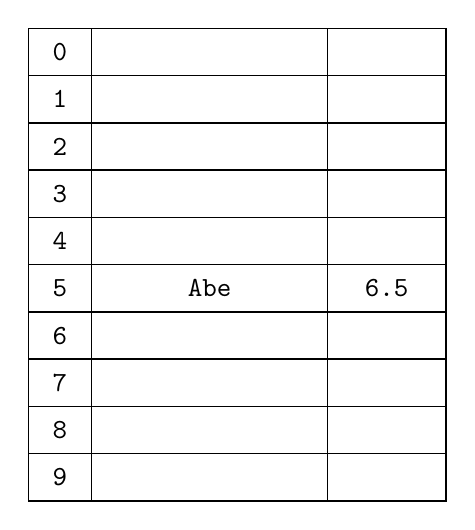
\begin{tikzpicture}

\draw (1.4, 0.7)
  node[draw, line width=0.02cm, , color=black,
       rounded corners=0cm, inner sep=0cm] {

\begin{minipage}[t][0.6cm]{0.8cm}
\mbox{}

\end{minipage}

};\draw (1.4, 0.7) node[color=black] {{\texttt{0}}};
\draw (3.3, 0.7)
  node[draw, line width=0.02cm, , color=black,
       rounded corners=0cm, inner sep=0cm] {

\begin{minipage}[t][0.6cm]{3.0cm}
\mbox{}

\end{minipage}

};\draw (3.3, 0.7) node[color=black] {{\texttt{}}};
\draw (5.55, 0.7)
  node[draw, line width=0.02cm, , color=black,
       rounded corners=0cm, inner sep=0cm] {

\begin{minipage}[t][0.6cm]{1.5cm}
\mbox{}

\end{minipage}

};\draw (5.55, 0.7) node[color=black] {{\texttt{}}};
\draw (1.4, 0.09999999999999987)
  node[draw, line width=0.02cm, , color=black,
       rounded corners=0cm, inner sep=0cm] {

\begin{minipage}[t][0.6cm]{0.8cm}
\mbox{}

\end{minipage}

};\draw (1.4, 0.09999999999999987) node[color=black] {{\texttt{1}}};
\draw (3.3, 0.09999999999999987)
  node[draw, line width=0.02cm, , color=black,
       rounded corners=0cm, inner sep=0cm] {

\begin{minipage}[t][0.6cm]{3.0cm}
\mbox{}

\end{minipage}

};\draw (3.3, 0.09999999999999987) node[color=black] {{\texttt{}}};
\draw (5.55, 0.09999999999999987)
  node[draw, line width=0.02cm, , color=black,
       rounded corners=0cm, inner sep=0cm] {

\begin{minipage}[t][0.6cm]{1.5cm}
\mbox{}

\end{minipage}

};\draw (5.55, 0.09999999999999987) node[color=black] {{\texttt{}}};
\draw (1.4, -0.5000000000000002)
  node[draw, line width=0.02cm, , color=black,
       rounded corners=0cm, inner sep=0cm] {

\begin{minipage}[t][0.6cm]{0.8cm}
\mbox{}

\end{minipage}

};\draw (1.4, -0.5000000000000002) node[color=black] {{\texttt{2}}};
\draw (3.3, -0.5000000000000002)
  node[draw, line width=0.02cm, , color=black,
       rounded corners=0cm, inner sep=0cm] {

\begin{minipage}[t][0.6cm]{3.0cm}
\mbox{}

\end{minipage}

};\draw (3.3, -0.5000000000000002) node[color=black] {{\texttt{}}};
\draw (5.55, -0.5000000000000002)
  node[draw, line width=0.02cm, , color=black,
       rounded corners=0cm, inner sep=0cm] {

\begin{minipage}[t][0.6cm]{1.5cm}
\mbox{}

\end{minipage}

};\draw (5.55, -0.5000000000000002) node[color=black] {{\texttt{}}};
\draw (1.4, -1.1000000000000003)
  node[draw, line width=0.02cm, , color=black,
       rounded corners=0cm, inner sep=0cm] {

\begin{minipage}[t][0.6cm]{0.8cm}
\mbox{}

\end{minipage}

};\draw (1.4, -1.1000000000000003) node[color=black] {{\texttt{3}}};
\draw (3.3, -1.1000000000000003)
  node[draw, line width=0.02cm, , color=black,
       rounded corners=0cm, inner sep=0cm] {

\begin{minipage}[t][0.6cm]{3.0cm}
\mbox{}

\end{minipage}

};\draw (3.3, -1.1000000000000003) node[color=black] {{\texttt{}}};
\draw (5.55, -1.1000000000000003)
  node[draw, line width=0.02cm, , color=black,
       rounded corners=0cm, inner sep=0cm] {

\begin{minipage}[t][0.6cm]{1.5cm}
\mbox{}

\end{minipage}

};\draw (5.55, -1.1000000000000003) node[color=black] {{\texttt{}}};
\draw (1.4, -1.7000000000000002)
  node[draw, line width=0.02cm, , color=black,
       rounded corners=0cm, inner sep=0cm] {

\begin{minipage}[t][0.6cm]{0.8cm}
\mbox{}

\end{minipage}

};\draw (1.4, -1.7000000000000002) node[color=black] {{\texttt{4}}};
\draw (3.3, -1.7000000000000002)
  node[draw, line width=0.02cm, , color=black,
       rounded corners=0cm, inner sep=0cm] {

\begin{minipage}[t][0.6cm]{3.0cm}
\mbox{}

\end{minipage}

};\draw (3.3, -1.7000000000000002) node[color=black] {{\texttt{}}};
\draw (5.55, -1.7000000000000002)
  node[draw, line width=0.02cm, , color=black,
       rounded corners=0cm, inner sep=0cm] {

\begin{minipage}[t][0.6cm]{1.5cm}
\mbox{}

\end{minipage}

};\draw (5.55, -1.7000000000000002) node[color=black] {{\texttt{}}};
\draw (1.4, -2.3000000000000003)
  node[draw, line width=0.02cm, , color=black,
       rounded corners=0cm, inner sep=0cm] {

\begin{minipage}[t][0.6cm]{0.8cm}
\mbox{}

\end{minipage}

};\draw (1.4, -2.3000000000000003) node[color=black] {{\texttt{5}}};
\draw (3.3, -2.3000000000000003)
  node[draw, line width=0.02cm, , color=black,
       rounded corners=0cm, inner sep=0cm] {

\begin{minipage}[t][0.6cm]{3.0cm}
\mbox{}

\end{minipage}

};\draw (3.3, -2.3000000000000003) node[color=black] {{\texttt{Abe}}};
\draw (5.55, -2.3000000000000003)
  node[draw, line width=0.02cm, , color=black,
       rounded corners=0cm, inner sep=0cm] {

\begin{minipage}[t][0.6cm]{1.5cm}
\mbox{}

\end{minipage}

};\draw (5.55, -2.3000000000000003) node[color=black] {{\texttt{6.5}}};
\draw (1.4, -2.9000000000000004)
  node[draw, line width=0.02cm, , color=black,
       rounded corners=0cm, inner sep=0cm] {

\begin{minipage}[t][0.6cm]{0.8cm}
\mbox{}

\end{minipage}

};\draw (1.4, -2.9000000000000004) node[color=black] {{\texttt{6}}};
\draw (3.3, -2.9000000000000004)
  node[draw, line width=0.02cm, , color=black,
       rounded corners=0cm, inner sep=0cm] {

\begin{minipage}[t][0.6cm]{3.0cm}
\mbox{}

\end{minipage}

};\draw (3.3, -2.9000000000000004) node[color=black] {{\texttt{}}};
\draw (5.55, -2.9000000000000004)
  node[draw, line width=0.02cm, , color=black,
       rounded corners=0cm, inner sep=0cm] {

\begin{minipage}[t][0.6cm]{1.5cm}
\mbox{}

\end{minipage}

};\draw (5.55, -2.9000000000000004) node[color=black] {{\texttt{}}};
\draw (1.4, -3.500000000000001)
  node[draw, line width=0.02cm, , color=black,
       rounded corners=0cm, inner sep=0cm] {

\begin{minipage}[t][0.6cm]{0.8cm}
\mbox{}

\end{minipage}

};\draw (1.4, -3.500000000000001) node[color=black] {{\texttt{7}}};
\draw (3.3, -3.500000000000001)
  node[draw, line width=0.02cm, , color=black,
       rounded corners=0cm, inner sep=0cm] {

\begin{minipage}[t][0.6cm]{3.0cm}
\mbox{}

\end{minipage}

};\draw (3.3, -3.500000000000001) node[color=black] {{\texttt{}}};
\draw (5.55, -3.500000000000001)
  node[draw, line width=0.02cm, , color=black,
       rounded corners=0cm, inner sep=0cm] {

\begin{minipage}[t][0.6cm]{1.5cm}
\mbox{}

\end{minipage}

};\draw (5.55, -3.500000000000001) node[color=black] {{\texttt{}}};
\draw (1.4, -4.1000000000000005)
  node[draw, line width=0.02cm, , color=black,
       rounded corners=0cm, inner sep=0cm] {

\begin{minipage}[t][0.6cm]{0.8cm}
\mbox{}

\end{minipage}

};\draw (1.4, -4.1000000000000005) node[color=black] {{\texttt{8}}};
\draw (3.3, -4.1000000000000005)
  node[draw, line width=0.02cm, , color=black,
       rounded corners=0cm, inner sep=0cm] {

\begin{minipage}[t][0.6cm]{3.0cm}
\mbox{}

\end{minipage}

};\draw (3.3, -4.1000000000000005) node[color=black] {{\texttt{}}};
\draw (5.55, -4.1000000000000005)
  node[draw, line width=0.02cm, , color=black,
       rounded corners=0cm, inner sep=0cm] {

\begin{minipage}[t][0.6cm]{1.5cm}
\mbox{}

\end{minipage}

};\draw (5.55, -4.1000000000000005) node[color=black] {{\texttt{}}};
\draw (1.4, -4.7)
  node[draw, line width=0.02cm, , color=black,
       rounded corners=0cm, inner sep=0cm] {

\begin{minipage}[t][0.6cm]{0.8cm}
\mbox{}

\end{minipage}

};\draw (1.4, -4.7) node[color=black] {{\texttt{9}}};
\draw (3.3, -4.7)
  node[draw, line width=0.02cm, , color=black,
       rounded corners=0cm, inner sep=0cm] {

\begin{minipage}[t][0.6cm]{3.0cm}
\mbox{}

\end{minipage}

};\draw (3.3, -4.7) node[color=black] {{\texttt{}}};
\draw (5.55, -4.7)
  node[draw, line width=0.02cm, , color=black,
       rounded corners=0cm, inner sep=0cm] {

\begin{minipage}[t][0.6cm]{1.5cm}
\mbox{}

\end{minipage}

};\draw (5.55, -4.7) node[color=black] {{\texttt{}}};
\end{tikzpicture}

\end{center}


Again an $A$ means \lq\lq checked $a$".
Now at this point (meaning at this state),
the TM just keep moving right whenever it sees an $a$ (without changing what is read)
until it reads a $b$:
\begin{center}
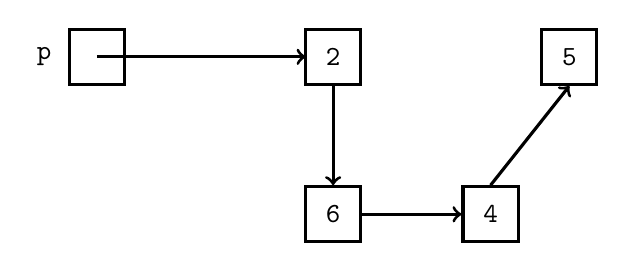
\begin{tikzpicture}

\draw (0.35, 0.35)
  node[draw, line width=0.04cm, , color=black,
       rounded corners=0cm, inner sep=0cm] {

\begin{minipage}[t][0.7cm]{0.7cm}
\mbox{}

\end{minipage}

};\draw (0.35, 0.35) node[color=black] {{\texttt{2}}};
\draw (0.35, -1.65)
  node[draw, line width=0.04cm, , color=black,
       rounded corners=0cm, inner sep=0cm] {

\begin{minipage}[t][0.7cm]{0.7cm}
\mbox{}

\end{minipage}

};\draw (0.35, -1.65) node[color=black] {{\texttt{6}}};
\draw (2.35, -1.65)
  node[draw, line width=0.04cm, , color=black,
       rounded corners=0cm, inner sep=0cm] {

\begin{minipage}[t][0.7cm]{0.7cm}
\mbox{}

\end{minipage}

};\draw (2.35, -1.65) node[color=black] {{\texttt{4}}};
\draw (3.35, 0.35)
  node[draw, line width=0.04cm, , color=black,
       rounded corners=0cm, inner sep=0cm] {

\begin{minipage}[t][0.7cm]{0.7cm}
\mbox{}

\end{minipage}

};\draw (3.35, 0.35) node[color=black] {{\texttt{5}}};\draw[line width=0.04cm,black,->] (0.35,-0.02) to  (0.35,-1.28);
\draw[line width=0.04cm,black,->] (0.72,-1.65) to  (1.98,-1.65);
\draw[line width=0.04cm,black,->] (2.35,-1.28) to  (3.35,-0.02);

\draw (-2.65, 0.35)
  node[draw, line width=0.04cm, , color=black,
       rounded corners=0cm, inner sep=0cm] {

\begin{minipage}[t][0.7cm]{0.7cm}
\mbox{}

\end{minipage}

};\draw (-2.65, 0.35) node[color=black] {{\texttt{}}};\draw[line width=0.04cm,black,->] (-2.65,0.35) to  (0,0.35);

\draw (-3.32, 0.35)
  node[draw, line width=0.04cm, , color=white,
       rounded corners=0cm, inner sep=0cm] {

\begin{minipage}[t][0.1cm]{0.1cm}
\mbox{}

\end{minipage}

};\draw (-3.32, 0.35) node[color=black] {{\texttt{p}}};
\end{tikzpicture}

\end{center}



At this point (meaning at this state), the TM replaces the $b$ with $B$ (in other words,
mark the $b$ as read), and move right by one step:
\begin{center}
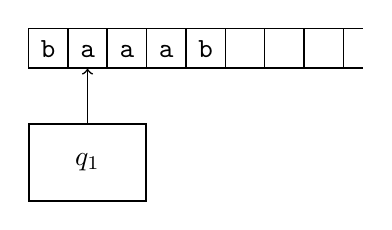
\begin{tikzpicture}

\draw (0.25, 0.25)
  node[draw, line width=0.02cm, , color=black,
       rounded corners=0cm, inner sep=0cm] {

\begin{minipage}[t][0.5cm]{0.5cm}
\mbox{}

\end{minipage}

};\draw (0.25, 0.25) node[color=black] {{\vphantom{baaab\SPACE\SPACE\SPACE}\texttt{b}}};
\draw (0.75, 0.25)
  node[draw, line width=0.02cm, , color=black,
       rounded corners=0cm, inner sep=0cm] {

\begin{minipage}[t][0.5cm]{0.5cm}
\mbox{}

\end{minipage}

};\draw (0.75, 0.25) node[color=black] {{\vphantom{baaab\SPACE\SPACE\SPACE}\texttt{a}}};
\draw (1.25, 0.25)
  node[draw, line width=0.02cm, , color=black,
       rounded corners=0cm, inner sep=0cm] {

\begin{minipage}[t][0.5cm]{0.5cm}
\mbox{}

\end{minipage}

};\draw (1.25, 0.25) node[color=black] {{\vphantom{baaab\SPACE\SPACE\SPACE}\texttt{a}}};
\draw (1.75, 0.25)
  node[draw, line width=0.02cm, , color=black,
       rounded corners=0cm, inner sep=0cm] {

\begin{minipage}[t][0.5cm]{0.5cm}
\mbox{}

\end{minipage}

};\draw (1.75, 0.25) node[color=black] {{\vphantom{baaab\SPACE\SPACE\SPACE}\texttt{a}}};
\draw (2.25, 0.25)
  node[draw, line width=0.02cm, , color=black,
       rounded corners=0cm, inner sep=0cm] {

\begin{minipage}[t][0.5cm]{0.5cm}
\mbox{}

\end{minipage}

};\draw (2.25, 0.25) node[color=black] {{\vphantom{baaab\SPACE\SPACE\SPACE}\texttt{b}}};
\draw (2.75, 0.25)
  node[draw, line width=0.02cm, , color=black,
       rounded corners=0cm, inner sep=0cm] {

\begin{minipage}[t][0.5cm]{0.5cm}
\mbox{}

\end{minipage}

};\draw (2.75, 0.25) node[color=black] {{\vphantom{baaab\SPACE\SPACE\SPACE}\texttt{\SPACE}}};
\draw (3.25, 0.25)
  node[draw, line width=0.02cm, , color=black,
       rounded corners=0cm, inner sep=0cm] {

\begin{minipage}[t][0.5cm]{0.5cm}
\mbox{}

\end{minipage}

};\draw (3.25, 0.25) node[color=black] {{\vphantom{baaab\SPACE\SPACE\SPACE}\texttt{\SPACE}}};
\draw (3.75, 0.25)
  node[draw, line width=0.02cm, , color=black,
       rounded corners=0cm, inner sep=0cm] {

\begin{minipage}[t][0.5cm]{0.5cm}
\mbox{}

\end{minipage}

};\draw (3.75, 0.25) node[color=black] {{\vphantom{baaab\SPACE\SPACE\SPACE}\texttt{\SPACE}}};\draw[line width=0.02cm,black] (4.0,0.5) to  (4.25,0.5);
\draw[line width=0.02cm,black] (4.0,0.0) to  (4.25,0.0);

\draw (0.75, -1.2)
  node[draw, line width=0.02cm, , color=black,
       rounded corners=0cm, inner sep=0cm] {

\begin{minipage}[t][0.98cm]{1.48cm}
\mbox{}

\end{minipage}

};\draw (0.75, -1.2) node[color=black] {$q_1$};\draw[line width=0.02cm,black,->] (0.75,-0.7) to  (0.75,-0.47) to  (0.75,-0.47) to  (0.75,-0.01);
\end{tikzpicture}

\end{center}



At this point, the TM moves to the right as long as it reads a $b$.
The TM will then reach this state:
\begin{center}
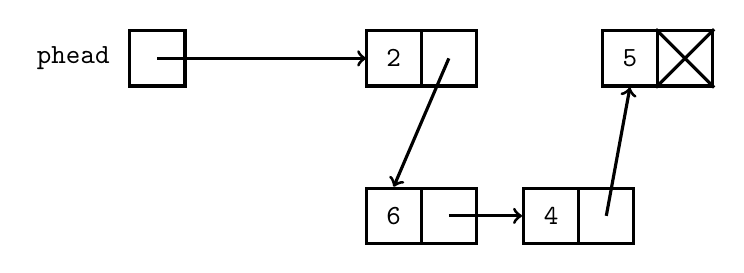
\begin{tikzpicture}

\draw (0.35, 0.35)
  node[draw, line width=0.04cm, , color=black,
       rounded corners=0cm, inner sep=0cm] {

\begin{minipage}[t][0.7cm]{0.7cm}
\mbox{}

\end{minipage}

};\draw (0.35, 0.35) node[color=black] {{\texttt{2}}};
\draw (1.0499999999999998, 0.35)
  node[draw, line width=0.04cm, , color=black,
       rounded corners=0cm, inner sep=0cm] {

\begin{minipage}[t][0.7cm]{0.7cm}
\mbox{}

\end{minipage}

};\draw (1.0499999999999998, 0.35) node[color=black] {{\texttt{}}};
\draw (0.35, -1.65)
  node[draw, line width=0.04cm, , color=black,
       rounded corners=0cm, inner sep=0cm] {

\begin{minipage}[t][0.7cm]{0.7cm}
\mbox{}

\end{minipage}

};\draw (0.35, -1.65) node[color=black] {{\texttt{6}}};
\draw (1.0499999999999998, -1.65)
  node[draw, line width=0.04cm, , color=black,
       rounded corners=0cm, inner sep=0cm] {

\begin{minipage}[t][0.7cm]{0.7cm}
\mbox{}

\end{minipage}

};\draw (1.0499999999999998, -1.65) node[color=black] {{\texttt{}}};
\draw (2.35, -1.65)
  node[draw, line width=0.04cm, , color=black,
       rounded corners=0cm, inner sep=0cm] {

\begin{minipage}[t][0.7cm]{0.7cm}
\mbox{}

\end{minipage}

};\draw (2.35, -1.65) node[color=black] {{\texttt{4}}};
\draw (3.0500000000000003, -1.65)
  node[draw, line width=0.04cm, , color=black,
       rounded corners=0cm, inner sep=0cm] {

\begin{minipage}[t][0.7cm]{0.7cm}
\mbox{}

\end{minipage}

};\draw (3.0500000000000003, -1.65) node[color=black] {{\texttt{}}};
\draw (3.35, 0.35)
  node[draw, line width=0.04cm, , color=black,
       rounded corners=0cm, inner sep=0cm] {

\begin{minipage}[t][0.7cm]{0.7cm}
\mbox{}

\end{minipage}

};\draw (3.35, 0.35) node[color=black] {{\texttt{5}}};
\draw (4.05, 0.35)
  node[draw, line width=0.04cm, , color=black,
       rounded corners=0cm, inner sep=0cm] {

\begin{minipage}[t][0.7cm]{0.7cm}
\mbox{}

\end{minipage}

};\draw (4.05, 0.35) node[color=black] {{\texttt{}}};\draw[line width=0.04cm,black,->] (1.05,0.35) to  (0.35,-1.28);
\draw[line width=0.04cm,black,->] (1.05,-1.65) to  (1.98,-1.65);
\draw[line width=0.04cm,black,->] (3.05,-1.65) to  (3.35,-0.02);
\draw[line width=0.04cm,black] (3.68,0.72) to  (4.42,-0.02);
\draw[line width=0.04cm,black] (4.42,0.72) to  (3.68,-0.02);

\draw (-2.65, 0.35)
  node[draw, line width=0.04cm, , color=black,
       rounded corners=0cm, inner sep=0cm] {

\begin{minipage}[t][0.7cm]{0.7cm}
\mbox{}

\end{minipage}

};\draw (-2.65, 0.35) node[color=black] {{\texttt{}}};\draw[line width=0.04cm,black,->] (-2.65,0.35) to  (0,0.35);

\draw (-3.7199999999999998, 0.35)
  node[draw, line width=0.04cm, , color=white,
       rounded corners=0cm, inner sep=0cm] {

\begin{minipage}[t][0.1cm]{0.1cm}
\mbox{}

\end{minipage}

};\draw (-3.7199999999999998, 0.35) node[color=black] {{\texttt{phead}}};
\end{tikzpicture}

\end{center}



The TM then reads $c$, replaces it with a $C$ and moves left by one.
\begin{center}
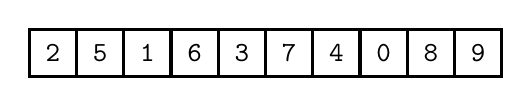
\begin{tikzpicture}

\draw (0.3, -0.3)
  node[draw, line width=0.04cm, , color=black,
       rounded corners=0cm, inner sep=0cm] {

\begin{minipage}[t][0.6cm]{0.6cm}
\mbox{}

\end{minipage}

};\draw (0.3, -0.3) node[color=black] {{\texttt{2}}};
\draw (0.8999999999999999, -0.3)
  node[draw, line width=0.04cm, , color=black,
       rounded corners=0cm, inner sep=0cm] {

\begin{minipage}[t][0.6cm]{0.6cm}
\mbox{}

\end{minipage}

};\draw (0.8999999999999999, -0.3) node[color=black] {{\texttt{5}}};
\draw (1.5, -0.3)
  node[draw, line width=0.04cm, , color=black,
       rounded corners=0cm, inner sep=0cm] {

\begin{minipage}[t][0.6cm]{0.6cm}
\mbox{}

\end{minipage}

};\draw (1.5, -0.3) node[color=black] {{\texttt{1}}};
\draw (2.0999999999999996, -0.3)
  node[draw, line width=0.04cm, , color=black,
       rounded corners=0cm, inner sep=0cm] {

\begin{minipage}[t][0.6cm]{0.6cm}
\mbox{}

\end{minipage}

};\draw (2.0999999999999996, -0.3) node[color=black] {{\texttt{6}}};
\draw (2.7, -0.3)
  node[draw, line width=0.04cm, , color=black,
       rounded corners=0cm, inner sep=0cm] {

\begin{minipage}[t][0.6cm]{0.6cm}
\mbox{}

\end{minipage}

};\draw (2.7, -0.3) node[color=black] {{\texttt{3}}};
\draw (3.3, -0.3)
  node[draw, line width=0.04cm, , color=black,
       rounded corners=0cm, inner sep=0cm] {

\begin{minipage}[t][0.6cm]{0.6cm}
\mbox{}

\end{minipage}

};\draw (3.3, -0.3) node[color=black] {{\texttt{7}}};
\draw (3.9, -0.3)
  node[draw, line width=0.04cm, , color=black,
       rounded corners=0cm, inner sep=0cm] {

\begin{minipage}[t][0.6cm]{0.6cm}
\mbox{}

\end{minipage}

};\draw (3.9, -0.3) node[color=black] {{\texttt{4}}};
\draw (4.5, -0.3)
  node[draw, line width=0.04cm, , color=black,
       rounded corners=0cm, inner sep=0cm] {

\begin{minipage}[t][0.6cm]{0.6cm}
\mbox{}

\end{minipage}

};\draw (4.5, -0.3) node[color=black] {{\texttt{0}}};
\draw (5.1, -0.3)
  node[draw, line width=0.04cm, , color=black,
       rounded corners=0cm, inner sep=0cm] {

\begin{minipage}[t][0.6cm]{0.6cm}
\mbox{}

\end{minipage}

};\draw (5.1, -0.3) node[color=black] {{\texttt{8}}};
\draw (5.699999999999999, -0.3)
  node[draw, line width=0.04cm, , color=black,
       rounded corners=0cm, inner sep=0cm] {

\begin{minipage}[t][0.6cm]{0.6cm}
\mbox{}

\end{minipage}

};\draw (5.699999999999999, -0.3) node[color=black] {{\texttt{9}}};
\end{tikzpicture}

\end{center}



The TM has nw finished one round of match one $a$, one $b$, and one $c$.

\[
\begin{tabular}{|c|c|l|}
  \hline
  $(q,x)$ & $\delta(q,x)$ & \mbox{} \\
  \hline
  $(q_0,a)$ & $(q_1,A,R)$ & Start marking phase: Mark $a$ and move right \\
  $(q_1,a)$ & $(q_1,a,R)$ & Fast forward over $a$ \\
  $(q_1,B)$ & $(q_1,B,R)$ & Fast forward over $B$ \\
  $(q_1,b)$ & $(q_2,B,R)$ & Mark $b$ and move right \\
  $(q_2,b)$ & $(q_2,b,R)$ & Fast forward over $b$ \\
  $(q_2,C)$ & $(q_2,C,R)$ & Fast forward over $C$ \\
  $(q_2,c)$ & $(q_3,C,L)$ & Mark $c$ and move left \\
  $(q_3,C)$ & $(q_3,C,L)$ & Rewind over $C$ \\
  $(q_3,B)$ & $(q_3,B,L)$ & Rewind over $B$ \\
  $(q_3,b)$ & $(q_3,b,L)$ & Rewind over $b$ \\
  $(q_3,a)$ & $(q_3,a,L)$ & Rewind over $a$ \\
  $(q_3,A)$ & $(q_0,A,R)$ & On seeing $A$, go to state $q_0$\\
  $(q_0,B)$ & $(q_4,B,R)$ & Start scanning phase: read first $B$ and move right\\
  $(q_4,B)$ & $(q_4,B,R)$ & Fast forward over $B$ \\
  $(q_4,C)$ & $(q_5,C,R)$ & Read first C and move right\\
  $(q_5,C)$ & $(q_5,C,R)$ & Fast forward over $C$\\
  $(q_5,\BLANK)$ & $(q_{\accept},B,S)$ & Accept string when a $\BLANK$ is found\\
  \hline
\end{tabular}
\]

Make sure you draw the state (or transition) diagram. Again
transitions which are not labeled go to the $q_{\reject}$ state.
Instead of writing infinitely many blanks, we will write one blank
just beyond $abc$. If we need to we can add blanks when we need to
(actually, for this TM only one blank is needed.)

Now let's trace the execution of $M$ for the string $abc$.
\begin{align*}
q_0 abc\BLANK
 &\derive Aq_1bc\BLANK \\
 &\derive ABq_2c\BLANK \\
 &\derive Aq_3BC\BLANK \\
 &\derive q_3ABC\BLANK \\
 &\derive Aq_0BC\BLANK \\
 &\derive ABq_4C\BLANK \\
 &\derive ABCq_5\BLANK \\
 &\derive ABCq_{\accept}\BLANK \\
\end{align*}

Now try to trace the execution of the TM for $aabbcc$ and
$aabbccc$.
\end{eg}

\begin{eg}
You can use TM to compute numbers. For instance you can use the
string $111$ to represent $3$. Given this data format, you can
define the output of a TM $M$ by what's on the tape when then
machine halts. Can you define a TM that computes the twice
function. In other words $M(111)$ = $111111$, i.e., if you put
$111$ on the tape and run the machine, it should halt with
$111111$ on the tape. If the TM does not halt on input $x$, then
we say $M(x)$ \defone{diverges}.
\begin{itemize}
 \item You can design a
 TM to add numbers. For instance to add two 3 and 5, the input to
 the TM is $\#111\#11111$. The expected output is $11111111$. Can
 you design such a TM?
\item Can you design one to perform subtract
 of the form $m-n$ where $m\geq n$? In otherwise you want to
 design a TM $M$ such that $M(\#11111\#11) = 111$.
 \item Can you design a TM to do multiplication? For instance to
 compute the product of 3 and 4, you run the machine with
 $111\#1111$ and get $M(111\#1111) = 111111111111$.
 \item Can you design a TM $M$ that can powers of 2? For instance
 $M(1) = 11$, $M(111) = 11111111$.
 \item Of course you can also compute rationals. For instance you
 can represent the fraction 3/4 by 11101111. Can you design a TM
 to add rationals?
 \item You can also model negative numbers just by using a special
 character for sign.
 \item Of course you can combine all the above into a single TM.
\end{itemize}
\end{eg}

\begin{eg} Here's a trick. To prevent the case where the TM moves
left while it's already at the leftmost position, you need to
shift all the character one position to the right. Suppose the
symbol $\#$ is not used. Suppose the TM is $M$. How would you
write a new TM that will shift the input by one space to the
right, put $\#$ as the first character, and move the read/write
head so that it's about to read the first character of the input
string (i.e., first character to the right of $\#$. Once this
pre-processing step is done, the new TM starts simulating the old
one. In other words in terms of ID, you want a TM $M'$ that will
do the following: Suppose the new start state is $q_0'$.
\[
 q_0x \derive \#q_0x
\]
Since this modification can always be carried out on any TM, in
many books, it's assumed that the TM will never fall off the left
edge. In other words, these authors assume that it the TM tries to
move left on the leftmost spot, it will simply stay and not move.
\end{eg}

\begin{eg}
Design a TM that accepts $\{a^nb^nc^n \,|\, n \equiv 1
\,\,\,(\operatorname{mod} \, 4)\}$. The solution is easy. First
the TM checks the input is of the form $a^nb^nc^n$. (We've already
done that). After this point if the $a$'s might be marked with
another character. Let's say it's been replaced by $A$'s. First
the TM go to the leftmost $A$. It moves right so that the
read/write head is reading the next $A$ (or possibly $B$). It will
then continually read 4 $A$'s until a $B$ is reached. If that can
be done, then TM enters the $q_{\accept}$ state. Otherwise it
enters the $q_{\reject}$ state.
\end{eg}


There are many other computational models ($\lambda$--calculus
random access machines, general recursive functions, etc.) But in
the end they are all proven to be only as powerful as the original
Turing machines. Therefore solving a problem algorithmically is
believed to be equivalent to solving a problem using a Turing
machine. This is known as the
\defone{Church-Turing thesis}.

\begin{eg}
In some books, a Turing machine is defined very similar to our
definition above except that the movements of the read/write head
is either left or right; the read/write head cannot stay at the
same spot. It seems that such a definition would result in a
weaker TM. Is that true?
\end{eg}

